\documentclass[11pt]{article}
\pdfminorversion=7
\usepackage[utf8]{inputenc}
\usepackage[T1]{fontenc}
\usepackage[english]{babel}
\usepackage{lmodern,microtype}
\usepackage[a4paper,margin=25mm]{geometry}
\usepackage{amsmath,amssymb,bm,graphicx,booktabs,array,tabularx}
\usepackage[round,authoryear]{natbib}
\usepackage{enumitem,placeins,xcolor}
\usepackage[colorlinks=true,linkcolor=blue!45!black,citecolor=blue!45!black,urlcolor=blue!45!black]{hyperref}
\usepackage{caption,xurl}
\captionsetup{font=small,labelfont=bf}
\setlength{\parskip}{4pt}
\setlength{\parindent}{1em}
\setlength{\emergencystretch}{2em}
\setlength{\textfloatsep}{16pt}
\renewcommand{\topfraction}{0.9}
\renewcommand{\bottomfraction}{0.8}
\renewcommand{\textfraction}{0.08}
\renewcommand{\floatpagefraction}{0.45}
\setcounter{topnumber}{3}
\setcounter{totalnumber}{5}
\raggedbottom
\graphicspath{{figures/}}
\newcommand{\E}{\operatorname{E}}
\newcommand{\Var}{\operatorname{Var}}
\newcommand{\diag}{\operatorname{diag}}

\hypersetup{pdftitle={Bayesian spectral learning on road networks},pdfauthor={}}

\renewcommand{\thesection}{S\arabic{section}}
\renewcommand{\thetable}{S\arabic{table}}
\renewcommand{\thefigure}{S\arabic{figure}}
\setlength{\parskip}{3pt}
\setlength{\textfloatsep}{9pt}
\setlength{\intextsep}{9pt}
\captionsetup{font=small,skip=4pt}
\begin{document}
\begin{center}\large\textbf{Supplementary material}\\[3pt]
\normalsize Bayesian spectral learning on road networks\end{center}
\section{Recorded categories and coefficients}
U denotes no attributes and fixed length; C includes attributes and fixed length; L includes attributes and estimates length. The retained supports contain 2,540 Barcelona and 6,079 Bogot\'a segments. Unknown labels describe missing recording, not absent infrastructure. Other surface tags include generic paved tags. A Bogot\'a lane count of 22 was assigned to unknown. Reference categories are residential roads, two lanes and asphalt.
\par
\begin{table}[!htbp]\centering\small
\caption{Recorded attribute categories on the retained support.}
\begin{tabular}{llrr}\toprule Attribute & Category & Barcelona & Bogot\'a\\\midrule
Road class & residential & 932 & 2658 \\
Road class & tertiary & 530 & 1377 \\
Road class & secondary & 800 & 1282 \\
Road class & primary & 278 & 762 \\
Lanes & two & 659 & 4260 \\
Lanes & one & 298 & 461 \\
Lanes & three\_plus & 1153 & 860 \\
Lanes & unknown & 430 & 498 \\
Surface tag & asphalt & 2380 & 5336 \\
Surface tag & other\_recorded & 22 & 583 \\
Surface tag & unknown & 138 & 160 \\
\bottomrule
\end{tabular}\end{table}
\FloatBarrier
\par

\par
\begin{table}[!htbp]\centering\small
\caption{Conditional count ratios in the mixture L models: medians and marginal 90\% intervals. Unknown-category coefficients are nuisance controls.}
\begin{tabular}{llrrr}\toprule Network & Indicator & Median ratio & 5th percentile & 95th percentile\\\midrule
Barcelona & Tertiary road & 1.14 & 0.95 & 1.35 \\
Barcelona & Secondary road & 0.97 & 0.80 & 1.18 \\
Barcelona & Primary road & 1.29 & 1.04 & 1.60 \\
Barcelona & One lane & 0.84 & 0.69 & 1.03 \\
Barcelona & Three or more lanes & 1.49 & 1.27 & 1.74 \\
Barcelona & Unknown lane count & 0.74 & 0.60 & 0.91 \\
Barcelona & Other surface tag & 0.86 & 0.52 & 1.48 \\
Barcelona & Unknown surface & 0.71 & 0.55 & 0.92 \\
Bogot\'a & Tertiary road & 1.95 & 1.78 & 2.13 \\
Bogot\'a & Secondary road & 2.59 & 2.36 & 2.84 \\
Bogot\'a & Primary road & 3.73 & 3.35 & 4.17 \\
Bogot\'a & One lane & 1.07 & 0.95 & 1.20 \\
Bogot\'a & Three or more lanes & 1.29 & 1.17 & 1.43 \\
Bogot\'a & Unknown lane count & 0.55 & 0.48 & 0.63 \\
Bogot\'a & Other surface tag & 0.82 & 0.73 & 0.92 \\
Bogot\'a & Unknown surface & 1.19 & 0.97 & 1.47 \\
\bottomrule
\end{tabular}\end{table}
\FloatBarrier
\par
\clearpage
\section{Sampling and predictive checks}
N denotes nonspatial NB, D dense spectral, M mixture spectral and B spectral BYM2. The joint criterion required no divergences or depth saturation, maximum $\widehat R\leq1.01$, minimum bulk ESS $\geq400$ and minimum E-BFMI $\geq0.3$. All retained fits had zero divergences and depth saturations. The four BYM2 fits retained energy warnings after longer runs; successful execution does not establish adequate exploration. Pointwise PSIS-LOO does not assess spatial transferability.
\par
\begin{table}[!htbp]\centering\small
\caption{Core sampler diagnostics. Minimum E-BFMI is across four chains; independent-effect checks also apply to BYM2.}
\begin{tabular}{llrrrrl}\toprule Network & Model & Draws/chain & Max. $\widehat R$ & Min. ESS & Min. E-BFMI & Criterion\\\midrule
Barcelona & B-C & 2000 & 1.006 & 442 & 0.246 & Flagged \\
Barcelona & B-U & 2000 & 1.012 & 386 & 0.203 & Flagged \\
Barcelona & D-C & 1000 & 1.005 & 946 & 0.738 & Pass \\
Barcelona & D-U & 1000 & 1.004 & 752 & 0.666 & Pass \\
Barcelona & N-C & 1000 & 1.002 & 1676 & 0.907 & Pass \\
Barcelona & N-L & 1000 & 1.002 & 1721 & 0.940 & Pass \\
Barcelona & N-U & 1000 & 1.002 & 1512 & 0.885 & Pass \\
Barcelona & M-C & 1000 & 1.004 & 1456 & 0.966 & Pass \\
Barcelona & M-L & 1000 & 1.003 & 1529 & 0.904 & Pass \\
Barcelona & M-U & 1000 & 1.004 & 1700 & 0.909 & Pass \\
Bogot\'a & B-C & 2000 & 1.006 & 376 & 0.191 & Flagged \\
Bogot\'a & B-U & 2000 & 1.004 & 700 & 0.277 & Flagged \\
Bogot\'a & D-C & 1000 & 1.004 & 921 & 0.771 & Pass \\
Bogot\'a & D-U & 1000 & 1.003 & 829 & 0.697 & Pass \\
Bogot\'a & N-C & 1000 & 1.002 & 1820 & 0.973 & Pass \\
Bogot\'a & N-L & 1000 & 1.001 & 1824 & 0.981 & Pass \\
Bogot\'a & N-U & 1000 & 1.002 & 1470 & 0.971 & Pass \\
Bogot\'a & M-C & 1000 & 1.004 & 1677 & 0.869 & Pass \\
Bogot\'a & M-L & 1000 & 1.003 & 1456 & 0.934 & Pass \\
Bogot\'a & M-U & 1000 & 1.005 & 1660 & 0.881 & Pass \\
\bottomrule
\end{tabular}\end{table}
\FloatBarrier
\par

\par
\begin{table}[!htbp]\centering\small
\caption{Mixture L predictive checks, using 400 replicated datasets. $p_+$ is the fraction of replicated statistics at least as large as observed.}
\begin{tabular}{llrrrl}\toprule Network & Statistic & Observed & Rep. median & 90\% rep. interval & $p_+$\\\midrule
Barcelona & Zero fraction & 0.540 & 0.536 & [0.513, 0.558] & 0.383 \\
Barcelona & Variance & 7.58 & 7.89 & [6.30, 10.68] & 0.595 \\
Barcelona & Maximum & 26.00 & 37.00 & [26.00, 71.10] & 0.958 \\
Barcelona & 99th percentile & 13.00 & 13.00 & [11.61, 15.00] & 0.675 \\
Barcelona & Mean & 1.470 & 1.443 & [1.324, 1.567] & 0.365 \\
Bogot\'a & Zero fraction & 0.283 & 0.249 & [0.237, 0.260] & 0.000 \\
Bogot\'a & Variance & 899.32 & 1034.85 & [795.81, 1406.34] & 0.795 \\
Bogot\'a & Maximum & 815.00 & 700.50 & [443.90, 1353.25] & 0.318 \\
Bogot\'a & 99th percentile & 146.22 & 146.00 & [131.21, 164.23] & 0.490 \\
Bogot\'a & Mean & 13.994 & 13.871 & [13.103, 14.851] & 0.412 \\
\bottomrule
\end{tabular}\end{table}
\FloatBarrier
\par
\clearpage
\section{Residual dependence and field uncertainty}
Residual checks used centred Pearson residuals on the reconstructed adjacency. Residual dependence remained outside replicated reference ranges. Improved scores and sampler convergence do not imply complete spatial or distributional adequacy. In particular, the Bogot\'a mixture L model underpredicted the zero fraction (Table S4).
\par
\begin{table}[!htbp]\centering\small
\caption{Residual Moran's $I$ for the estimated-length models. Values use centred Pearson residuals and the reconstructed segment adjacency; the replicated reference is conditional on each draw.}
\begin{tabular}{llrrrl}\toprule Network & Model & Observed median & Rep. median & 90\% rep. interval & $p_+$\\\midrule
Barcelona & N-L & -0.046 & -0.003 & [-0.020, 0.025] & 1.00 \\
Barcelona & M-L & -0.055 & 0.001 & [-0.028, 0.025] & 1.00 \\
Bogot\'a & N-L & 0.118 & 0.000 & [-0.019, 0.016] & 0.00 \\
Bogot\'a & M-L & 0.089 & -0.002 & [-0.013, 0.013] & 0.00 \\
\bottomrule
\end{tabular}\end{table}
\FloatBarrier
\par

The structured field combines all 20 candidate coefficients, including coefficients predominantly allocated to the continuous spike. Marginal interval sign support does not imply simultaneous hotspot significance or traffic-adjusted risk.
\par
\begin{figure}[!htbp]\centering
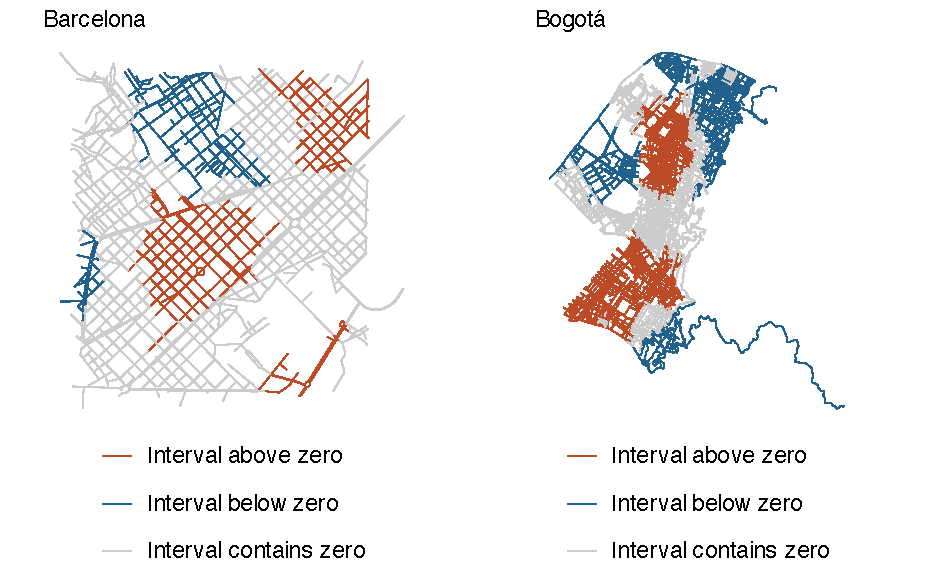
\includegraphics[width=\textwidth]{field_uncertainty.pdf}
\caption{Marginal 90\% structured-field intervals in mixture L fits. Colours distinguish intervals above, below or containing zero. These segment-wise summaries differ from component slab membership.}
\end{figure}
\FloatBarrier
\par

\noindent\textbf{Scope.} These tables concern the revised ordered prior and four-chain empirical fits. Source-record reconstruction reproduced the model inputs exactly while preserving report-row and person-involvement counting units. Temporal alignment of attributes, sensitivity to priors and basis dimension, harmonized simulation and spatially blocked validation remain outstanding.
\end{document}
